In this section we explore the effect of varying the underlying binary physics assumptions and the model for the Milky Way. In Section~\ref{sec:detection_rate_analysis} we explore the changes in the detection rate over different physics variations  and in Section~\ref{sec:property_variations} we consider how these model physics variations change the properties of detectable systems. Finally we demonstrate how different models for the Milky Way can affect our results in Section~\ref{sec:mw_changes}.

\subsection{Detection rates}\label{sec:detection_rate_analysis}
\tom{I will be updating this section once the other physics variations are done running. There will be a couple of new models and the current ones will have better high Z resolution.}

We find that for our fiducial model on average, a 4-year LISA mission will detect \BHBHFourYear{} BHBHs, \BHNSFourYear{} BHNSs and \NSNSFourYear{} NSNSs. Increasing to a 10-year LISA mission length changes the number of detections to \BHBHTenYear{}, \BHNSTenYear{} and \NSNSTenYear{} respectively. In Figure~\ref{fig:detection_rates}, we show the expected number of LISA detections for each model variation and discuss the prominent trends in the following sections. We show the rates and uncertainties plotted in this figure in Table~\ref{tab:detection_rates}.

\begin{figure*}[p]
    \centering
    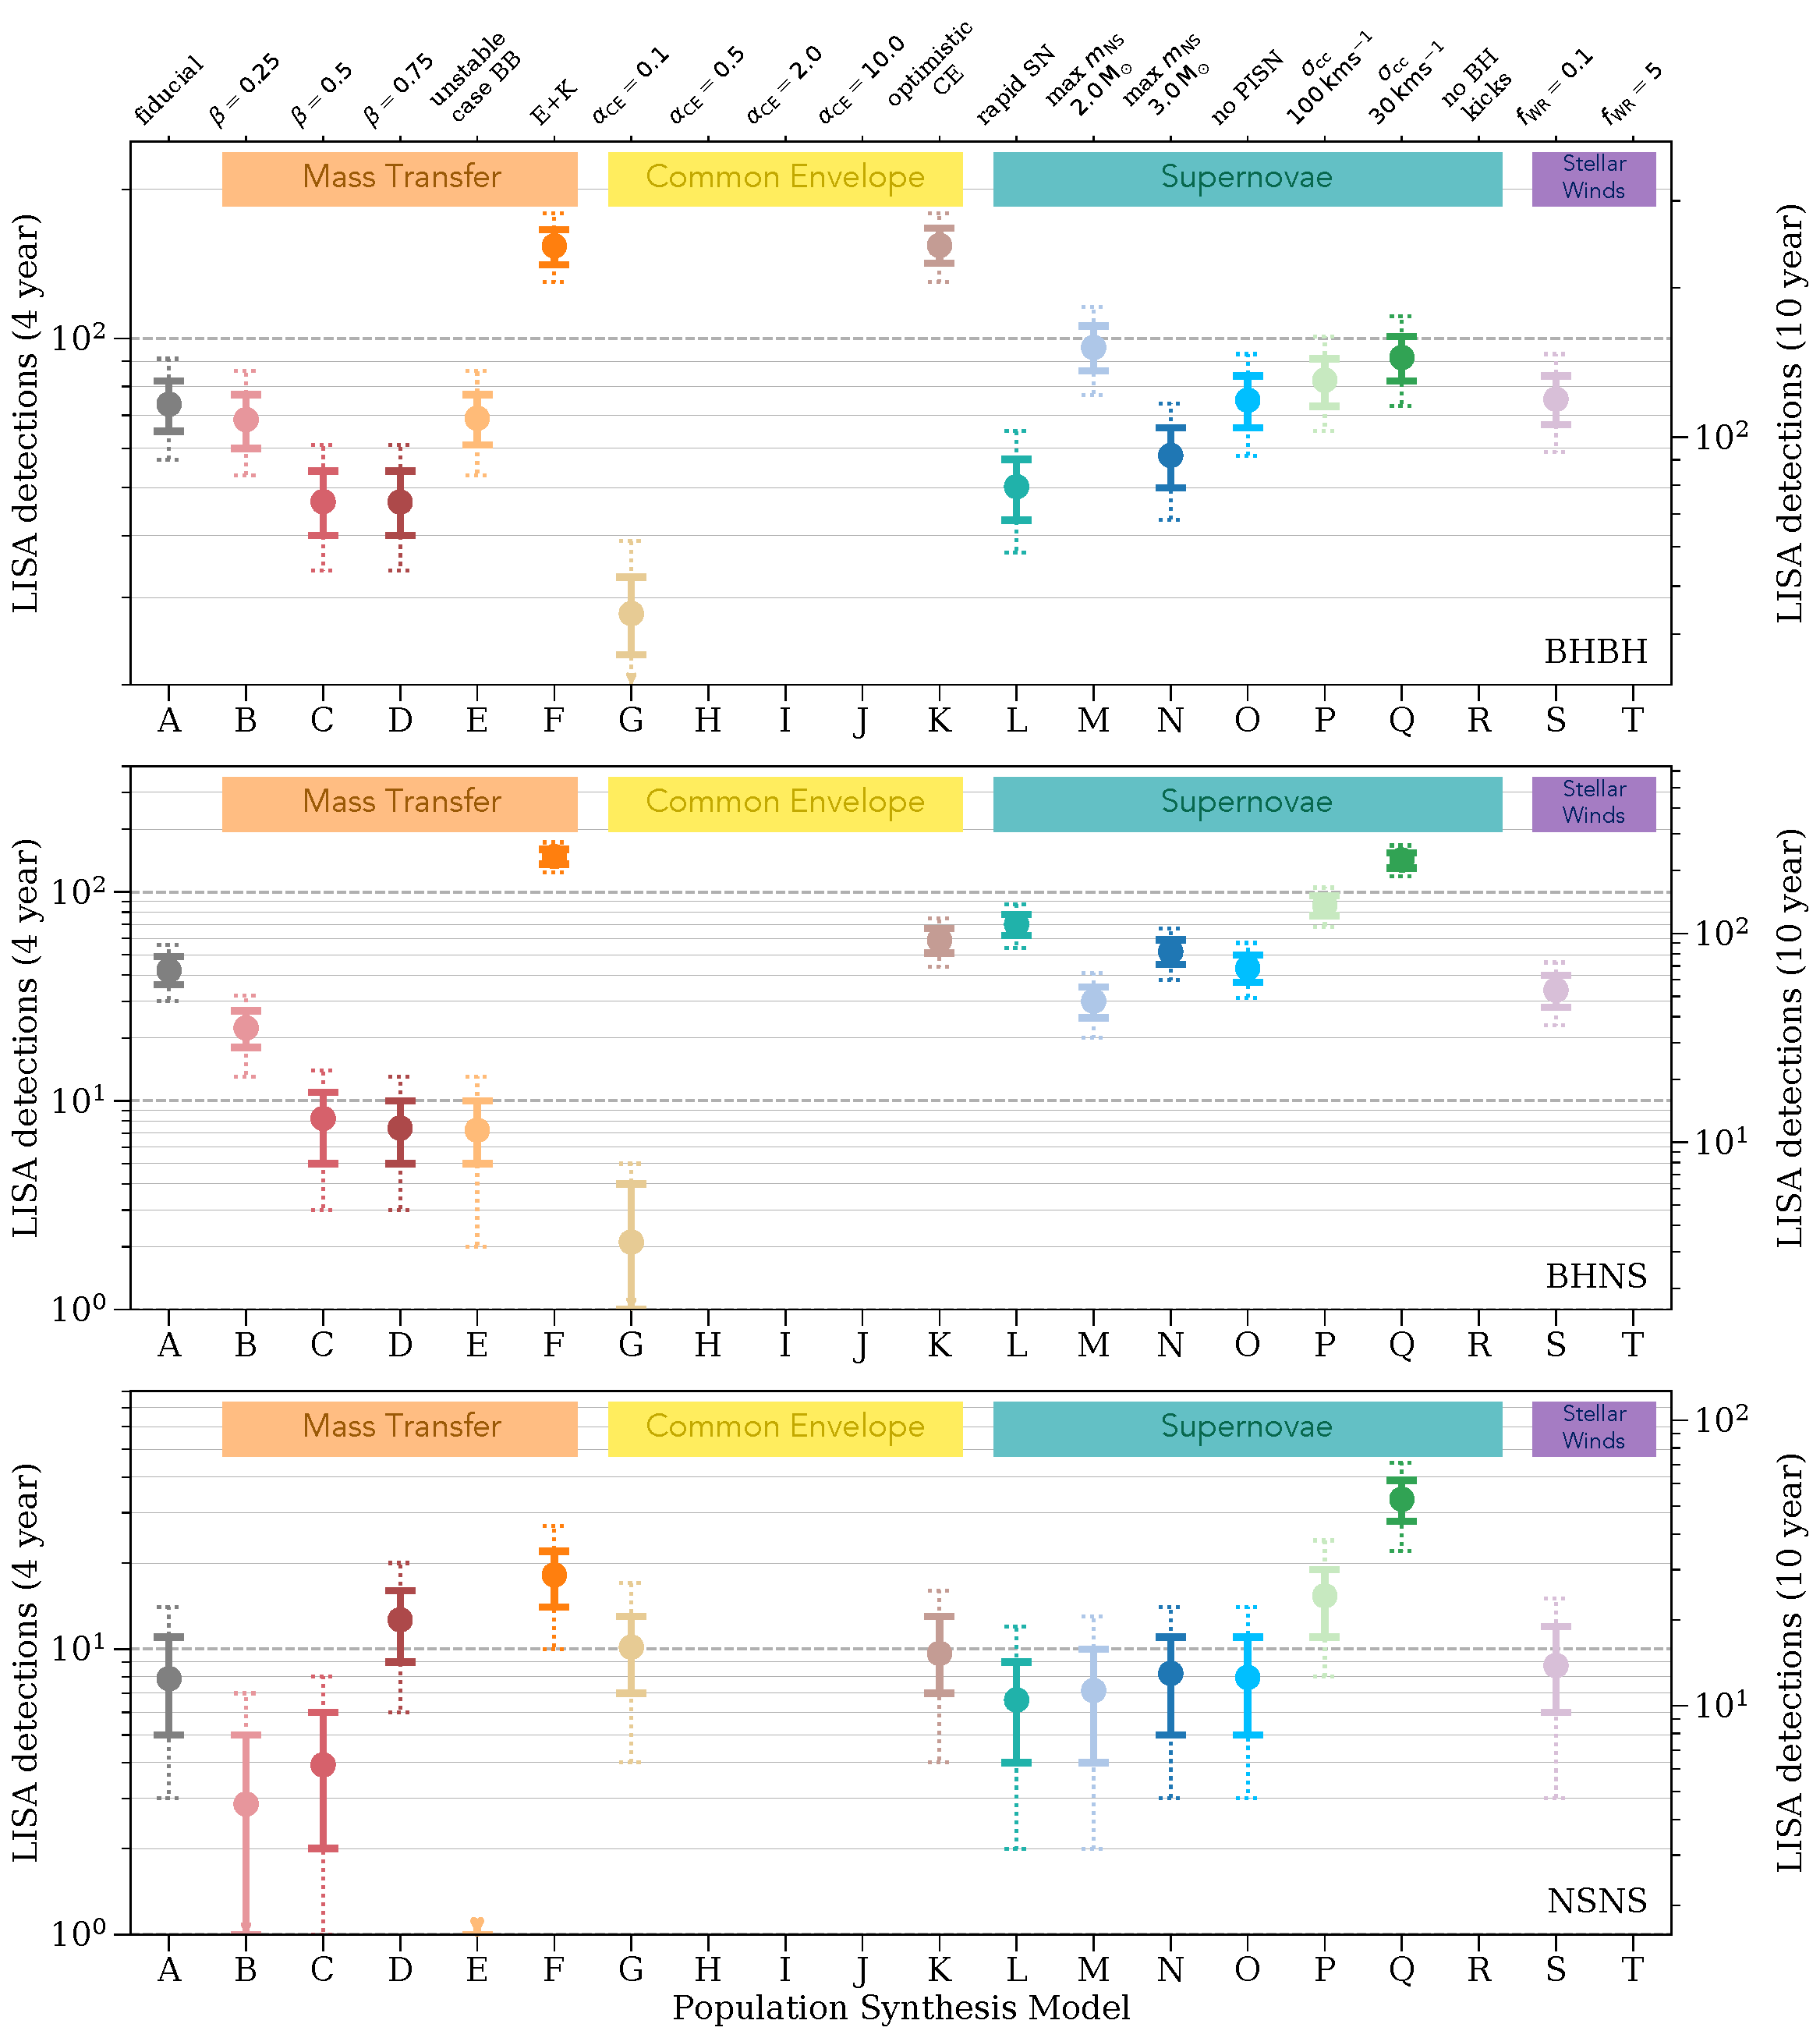
\includegraphics[width=\textwidth]{3_dco_detections.pdf}
    \caption{The number of expected detections in the LISA mission for different DCO types and model variations. Error bars show the 1- (solid) and 2-$\sigma$ (dotted) Poisson uncertainties. An arrow indicates that the error bar extends to zero. The left axis and grid lines show the number of detections in a 4-year LISA mission and the right axis shows an approximation of the number of detections in a 10-year mission (we scale the axis by $\sqrt{T_{\rm obs}}$, see Table~\ref{tab:detection_rates} for exact rates). Each model is described in further detail in Table~\ref{tab:physics_variations} and details of the fiducial assumptions are in Section~\ref{sec:fiducial_physics}. See Sec.~\ref{sec:detection_rate_analysis} for a discussion. \todo{Will add H, I, J, R, T once Floor says that they are done}}
    \label{fig:detection_rates}
\end{figure*}

\subsubsection{BHBH detection rate trends}
The BHBH detection rate is markedly robust across physics variations, with the expected detections in each model staying within 25\% of the fiducial rate (with the exception of model \modOpt{}). Thus even if there are changes in our understanding of the underlying physics before the LISA mission commences, the expected BHBH detection rate is unlikely to change significantly.

The exception to this statement is model \modOpt{}, in which we allow Hertzsprung gap donors to survive common envelope events. A large fraction of the progenitors of BHs in this mass range expand significantly during the Hertzsprung gap phase and initiate common envelope events. Therefore, though the detectable fraction does not change significantly, the increased population of BHBHs in the Milky Way leads to this model predicting 2.5 times more detections.

\subsubsection{BHNS detection rate trends}
In contrast, the BHNS detection rate is very sensitive to changes in binary physics assumptions. Therefore, once LISA flies and we know the actual number of detections, we can compare to each model and possibly provide some constraint on binary evolution physics. There are several notable trends in the BHNS detection rate in the middle pane of Figure~\ref{fig:detection_rates}.

As $\beta$ increases in models \modBetaLow{}-\modBetaHigh{}, the BHNS detection rate steadily decreases. This may seem unintuitive since a higher mass transfer efficiency should lead to more massive compact objects and thus a more detectable population. However, one must also consider that most of these DCOs are formed through a common envelope event and so retaining more of the envelope during mass transfer means that the eventual ejection of the envelope is much more difficult, thus leading to more stellar mergers and fewer detectable BHNSs \citep[e.g.][]{Kruckow+2018}.

\tom{@ALL, the trend with common envelopes still confuses me, specifially, why does it not increase when $\alpha=2.0$? We never quite resolved this in the thread in zpro\_tom\_wagg with me and Lieke. I do see that the BHBH have a lot of only stable mass transfer and so reasonably are not too affected. NSNS basically only come through CE events and so sensibly are strongly affected but BHNS have $\sim 70\%$ classic channel and so should be affected strongly. But we don't see an increase with $\alpha = 2.0$. Any thoughts? (I'm leaving thinking about this for now in case it changes with the new data haha)}
% For a similar reason, the rate is decreased when $\alpha$ is decreased in model \modAlphaLow{}, as this reduces the amount of orbital energy that is used to eject the envelope and thus leads to more stellar mergers. \todo{Why isn't the opposite true for model \modAlphaHigh{}? It seems the number of bound DCOs \textit{does} increase but the merging total decreases...?}

Enforcing that case BB mass transfer is always unstable (model \modCaseBB{}) decreases the detection rate as fewer NSs are produced and thus fewer BHNSs form. This is explained in further detail in Section~\ref{sec:NSNS_detection_trends}. For the same reason as the BHBH rate, model \modOpt{} has a higher number of detections. This change is less prominent than in the BHBH case as the progenitors tend to be lower masses and initiate a CE event less frequently during the Hertzsprung gap phase. 

The Fryer \textit{rapid} prescription (model \modRapid{}) leads to a higher detection rate for BHNSs because progenitors that would become black holes in the \textit{delayed} prescription, instead become neutron stars and so more BHNSs are formed instead of BHBHs. For the same reason, increasing the maximum neutron star mass (model \modNSHigh{}) increases the detection rate and the inverse is true when it is decreased (model \modNSLow{}).

Finally, models \modSigLow{}-\modNoBH{} show increased detection rates since lower kicks result in fewer disrupted binaries and hence a more numerous detectable population. Following this logic it makes sense that model \modSigLower{} produces more detections than model \modSigLow{}. The model with no BH kick (\modNoBH{}) is slightly lower than model \modSigLower{} as the number of surviving binaries is limited by the neutron star kick more than the black hole kick.

\subsubsection{NSNS detection rate trends}\label{sec:NSNS_detection_trends}

As $\beta$ increases the NSNS detection rate increases, the opposite trend to that seen in the BHNS rate. This is for two main reasons: firstly the ejection of a common envelope is less problematic for the less massive NSNS binaries. Moreover, the increased mass transfer efficiency means that systems that were previously below the mass necessary to become a NS can now accrete enough mass to form a NS. Although the same is true for more massive stars becoming BHs instead of NSs, due to the IMF, there is a net flux of more stars becoming NSs.

There is a drastic decrease in detections for model \modCaseBB{} by nearly two orders of magnitude. This is because the majority of NSNS binaries are formed through case BB mass transfer and setting this mass transfer to be always unstable results in many of these binaries to merge before they could become NSNSs. As a result the total number of detections decreases, however, interestingly the remaining population represent more massive progenitors (that would not go through case BB mass transfer) and thus is skewed to higher masses and has a \textit{higher} detectable fraction.

The vast majority of NSNSs in our sample are formed through the common envelope channel and thus changing the value of $\alpha_{\rm CE}$ has an effect on the rate. We see that decreasing $\alpha_{\rm CE}$ (model \modAlphaLow) leads to a lower rate as there is less energy available to eject the envelope and so more binaries result to stellar mergers rather than NSNSs and similarly we see an inverse trend when increasing $\alpha_{\rm CE}$ (model \modAlphaHigh).

As we found in the BHNS trends, a lower value for the core-collapse supernova velocity dispersion increases the detection rate in models \modSigLow{} and \modSigLower{}, whilst changing the PISN or BH kick prescription (models \modNoPISN{} and \modNoBH{}) of course has no effect on the NSNS population.

\subsection{Properties of detectable systems}\label{sec:property_variations}
\tom{This will be about how the shapes of the parameter distributions change for the different model variations. I won't detail every variation but I'll point out anything that stands out and leave the rest in the appendix plots.}
